\documentclass[11pt]{article}

\usepackage[utf8]{inputenc}
\usepackage[top=1.7in, bottom=1.5in, left=1in, right=1in]{geometry}
\usepackage{graphicx}
\usepackage{float}
\usepackage[usenames,dvipsnames]{xcolor}
\usepackage[hidelinks]{hyperref}
\usepackage{listings}
\lstset{
  breaklines=true,
  postbreak=\raisebox{0ex}[0ex][0ex]{\ensuremath{\color{gray}\hookrightarrow\space}}
}
\usepackage{caption}
\usepackage[ruled,vlined,linesnumbered]{algorithm2e}
\usepackage{mathtools}
\DeclarePairedDelimiter{\floor}{\lfloor}{\rfloor}
\usepackage[T1]{fontenc}
\usepackage{pgfplots}

\pgfplotsset{
  compat=newest,
  xlabel near ticks,
  ylabel near ticks
}

\newcommand{\localtextbulletone}{\textcolor{gray}{\raisebox{.45ex}{\rule{.6ex}{.6ex}}}}
	\renewcommand{\labelitemi}{\localtextbulletone}

\title{\textbf{Tweaking MINIX 3.1.5}}
\author{Hans Henrik Grønsleth, 14031693\\
		U08225 Foundations of Operating Systems}
\begin{document}

\maketitle
\tableofcontents

\clearpage
\section{Prerequisites}
All tests were performed on a virtual machine with a base memory of 128MB, created using VirtualBox 4.3\footnote{https://virtualbox.org}. The virtual machine was hosted on a HP Folio 13, 3.8GB memory, 4 x Intel® Core™ i5-2467M CPU @ 1.60GHz, 64-bit laptop running Ubuntu 14.04. The virtual machine only had access to 1 processor.

Booting the downloaded MINIX 3.1.5 image\footnote{http://wiki.minix3.org/doku.php?id=www:download:previousversions} from the VirtualBox GUI caused a kernel panic. This is due to a known problem of running MINIX on VirtualBox 4.x. The solution was to start the VM from the terminal using the following command:\\

\tt VBoxSDL --startvm minix --norawr0 --norawr3\normalfont\\\\
This disables raw rings 0 and 3 and did the trick.\footnote{http://wiki.minix3.org/doku.php?id=usersguide:runningonvirtualbox} The installation of MINIX was done according to the user guide\footnote{http://wiki.minix3.org/doku.php?id=usersguide:doinginstallation\#runningsetup}.

\section{Memory management}
\subsection{Test program}
To test changes done to MINIX's memory management, a memory test program was developed. The test program takes two inputs; (i) the number of processes to fork and (ii) the size of memory each process should take up. Each child process creates an array of the given size a number of times, and manipulates each entry of the array to make sure the memory is actually taken up. The program waits for all child processes to finish before exiting, this to make it easy to time how long it takes for the set of processes to finish. The full code with explaining comments can be found in Appendix \ref{app:memory_program}.

\subsection{Best Fit algorithm}
The Best Fit algorithm aims to find the smallest big enough hole when a process requires some memory. Below is a pseudo code of my implementation. The actual code can be found in Appendix \ref{app:alloc}.\\

\begin{algorithm}[H]
	\KwData{Required hole size}
	\KwResult{Pointer to smallest big enough free hole}
	Let $holes$ be the list of free holes\\
	$candidate\_hole \leftarrow holes[0]$;\\
	\ForEach{$hole$ in $holes$}{
		\If{hole size $>=$ required hole size {\bf and} hole size $<$ candidate\_hole size}{
	    $candidate\_hole$ = $hole$;
		}
	}
	\KwRet{Pointer to $candidate\_hole$}
	\caption{The Best Fit algorithm}
\end{algorithm}

\subsection{Quick Fit algorithm}
The Quick Fit algorithm aims to streamline the allocation of memory by keeping a cache of free blocks, based on their sizes. More specifically, a main list (a table) containing sublists is defined, where each sublist contains free holes of a certain size. When dealing with a request for a given size of memory, the algorithm returns a hole from the appropriate list. Unlike the Best Fit algorithm, Quick Fit does not have to search through the lists, it can simply return the last hole.

We have chosen to use 4 lists, each containing holes in a range of 8KB as listed in Table \ref{tab:list_sizes}. Three functions have been added to the file\\
\tt /usr/src/servers/vm/alloc.c\normalfont:

\begin{lstlisting}[language=c]
  void init_quick_fit_table(void){...};
  void assign_hole_to_list(struct hole *h) {...};
  void add_hole_to_list(struct quick_fit_list *qfl,
                        struct hole *h) {...};
  phys_clicks pop_hole_from_list(struct quick_fit_list *qfl) {...};
  
\end{lstlisting}
With the values given in Table \ref{tab:list_sizes}, we assign holes to lists by simply dividing the hole size ($h\_len$ in the code) by 8. This is possible because when dividing an int by an int, the floor function is used. I.e., $7/8$ produces 0, not 0.875. This gives us a nifty way of finding the index of the wanted list in the quick fit table. A hole of size 7 is referenced in List 0 $(\floor{7/8}=0)$, a hole of size 8 is referenced in List 1 $(\floor{8/8}=1)$, a hole of size 31 is referenced in List 3 $(\floor{31/8}=3)$etc. All holes of size $>=32$ are referenced in List 3.

When a request for a hole is placed, we use the same technique to determine which list to get the hole from; check whether the requested hole size is greater than 32, if 'yes' get hole from List 3, if 'no' get hole from list at index $requested\_hole\_size \over 8$ in the quick fit table.

\emph{Note: The implementation lacks a fallback mechanism for when there are no more available holes in a list. In this case, a hole from the next list (containing holes of greater sizes) should be returned.}

\begin{table}[H]
	\begin{center}
		\begin{tabular}{ r | l }
		List 0 & 0-8KB\\
		List 1 & 8-16KB\\
		List 2 & 16-32KB\\
		List 3 & 32KB$\rightarrow$
		\end{tabular}
	  
	  \caption{Memory sizes of quick fit lists}
	  \label{tab:list_sizes}
	\end{center}
\end{table}

\subsection{MINIX modifications}
The memory allocation algorithm in MINIX 3.1.5 is implemented in \\
\tt/usr/src/servers/vm/alloc.c\normalfont. The algorithms described above have been implemented alongside the original First Fit algorithm, and a switch-case statement have been added, encapsulating the three different algorithms to ease changing between them. An algorithm is selected by setting the variable \tt alloc\_algorithm \normalfont to 0 (First Fit), 1 (Best Fit) or 2 (Quick Fit). If other values are found the system uses First Fit. Sections that contain modified code can be found in Appendix \ref{app:alloc}. The file in its entirety can be found in the GitHub repository \cite{github}, where modifications are encapsulated by comments in the following way:\\
\begin{lstlisting}[language=c]
  /* ## start tweak ## */
  /* the modified code */
  /* ## end tweak ## */
\end{lstlisting}

\subsection{Test values}
To see how the different memory allocation algorithms affected the system, we wanted to test how each algorithm handled different number of processes taking up different sizes of memory.

We limit the experiments to explore three different numbers of processes; few, some and many, and three different memory size; small, medium and large. Throughout the experiments dealing with memory management, the values given in Table \ref{tab:number_of_processes_testing_memory} and Table \ref{tab:memory_sizes} were used to represent the number of processes running and sizes of memory being manipulated, respectively. We use 45 processes to represent many, as when ~60 processes are run simultaniously, the process table starts to fill up, which might have distorted the test results.

\begin{table}[H]
	\begin{minipage}{.5\textwidth}
		\begin{center}
			\begin{tabular}{ r | l }
			Few & 3\\
			Some & 15\\
			Many & 45
			\end{tabular}
		
			\caption{Number of processes}
			\label{tab:number_of_processes_testing_memory}
		\end{center}
	\end{minipage}
	\begin{minipage}{.5\textwidth}
		\begin{center}
			\begin{tabular}{ r | l }
			Small & 100B\\
			Medium & 10000B\\
			Large & 100000B
			\end{tabular}
			
			\caption{Memory sizes}
			\label{tab:memory_sizes}
		\end{center}
	\end{minipage}
\end{table}

\subsection{Testing processes with similar memory sizes}
Given that all processes take up the same size of memory, three possible numbers of processes and three possible memory sizes gives us $ 3 \times 3 = 9 $ scenarios to test; (1) few processes allocating (a) small, (b) medium and (c) large memory sizes, and similarly for (2) some and (3) many processes. Each scenario was run at least 3 times to get an average value, and major deviations were disregarded. Average times are given in Table \ref{tab:memory_results_similar}, best time in \emph{\color{MidnightBlue}blue}, worst in \emph{\color{BrickRed}red}.

\begin{table}[H]
	\begin{center}
		\begin{tabular}{ r | c | c | l }
		{ \bf \# of processes} & { \bf memory size } & { \bf algorithm } & { \bf time [s] }\\
		\hline
		   & 				& First Fit	& {\color{MidnightBlue}0.02}\\
		   & 100		& Best Fit	& 0.03\\
		   & 				& Qucik Fit	& 0.03\\ \cline{2-4}
		   & 				& First Fit	& {\color{MidnightBlue}0.22}\\
		3  & 10000	& Best Fit	& 0.32\\
		   & 				& Qucik Fit	& 0.32\\ \cline{2-4}
		   & 				& First Fit	& {\color{MidnightBlue}2.13}\\
		   & 100000	& Best Fit	& {\color{BrickRed}3.01}\\
		   & 				& Qucik Fit	& 3.00\\ \cline{2-4}
    \hline
		   & 				& First Fit	& 0.08\\
		   & 100		& Best Fit	& {\color{BrickRed}0.09}\\
		   & 				& Qucik Fit	& 0.08\\ \cline{2-4}
		   & 				& First Fit	& {\color{MidnightBlue}1.12}\\
		15 & 10000	& Best Fit	& 1.53\\
		   & 				& Qucik Fit	& 1.53\\ \cline{2-4}
		   & 				& First Fit	& {\color{MidnightBlue}14.69}\\
		   & 100000	& Best Fit	& 14.82\\
		   & 				& Qucik Fit	& {\color{BrickRed}15.00}\\ \cline{2-4}
    \hline
		   & 				& First Fit	& {\color{MidnightBlue}0.16}\\
		   & 100		& Best Fit	& {\color{BrickRed}0.22}\\
		   & 				& Qucik Fit	& 0.21\\ \cline{2-4}
		   & 				& First Fit	& {\color{MidnightBlue}3.33}\\
		45 & 10000	& Best Fit	& 4.58\\
		   & 				& Qucik Fit	& {\color{BrickRed}4.61}\\ \cline{2-4}
		   & 				& First Fit	& {\color{MidnightBlue}42.68}\\
		   & 100000	& Best Fit	& {\color{BrickRed}45.60}\\
		   & 				& Qucik Fit	& 44.88\\
    \hline
		\end{tabular}
	  
	  \caption{Memory test results: Similar array sizes}
	  \label{tab:memory_results_similar}
	\end{center}
\end{table}


\subsection{Testing processes with mixed memory sizes}
However, it might not always be the case that all processes take up the same amount of memory. To account for this, we modified our memory test program to start three sets of processes, where the first set takes a small piece of memory, the second a medium piece and the third set a large piece. Each scenario was run at least 3 times to get an average value, and major deviations were disregarded. Average times are given in Table \ref{tab:memory_results_mix}, best time in \emph{\color{MidnightBlue}blue}, worst in \emph{\color{BrickRed}red}.

\begin{table}
	\begin{center}
		\begin{tabular}{ r | c | l }
		{ \bf \# of processes} & { \bf algorithm } & { \bf time [s] }\\
		\hline
		   & First Fit & {\color{BrickRed}1.15}\\
		3  & Best Fit	 & {\color{MidnightBlue}1.11}\\
		   & Quick Fit & 1.12\\
    \hline
		   & First Fit & {\color{BrickRed}5.61}\\
		15 & Best Fit  & {\color{MidnightBlue}5.50}\\
		   & Quick Fit & 5.59\\
		\hline
		   & First Fit & {\color{BrickRed}16.73}\\
		45 & Best Fit  & 16.50\\
		   & Quick Fit & {\color{MidnightBlue}16.46}\\
		\end{tabular}
	  
	  \caption{Memory test results: Mixed array sizes}
	  \label{tab:memory_results_mix}
	\end{center}
\end{table}

\subsection{Discussion}
The results suggests that many processes using different sizes of memory suites Quick Fit well, while the overhead caused by the Best Fit and Quick Fit algorithms makes First Fit be the choice if all running processes use the same amount of memory. Best Fit should be preferred if there is a mix of memory sizes, but not too many processes running.

\section{Process management}
\subsection{Test program}
In order to test changes done to MINIX's process management, a process test program was developed. The test program takes one input; the number of processes to fork. Each child process calculates the number of primes less than 100 000 using the Sieve of Eratosthenes algorithm. Similar to the memory test program, the program waits for all child processes to finish before exiting in order to make it easy to time how long it takes for the set of processes to finish. The full code with explaining comments can be found in Appendix \ref{app:process_program}.

\subsection{MINIX modifications}
The quantum size in MINIX 3.1.5 is set in \tt/usr/src/kernel/table.c\normalfont. To carry out the experiments we simply change the \emph{qs} value for \emph{INIT\_PROC\_NR} to the desired value. This will affect all initiated processes, since they are all children of \tt init\normalfont.

\subsection{Test values}
The default quantum size of MINIX 3.1.5 is set to 8. A reasonable approach is to test sizes that are slightly smaller and larger, and see how this affects the system. We chose to test the system with the following quantum sizes: 2, 4, 8, 16, 32 and 64. Each quantum size was tested with a number of processes running at the same time. As with the testing of memory management, we chose to divide the number of processes into three; few, some and many. The values used are given in Table \ref{tab:number_of_processes_testing_quantum}. Each scenario was run at least 3 times to get an average value, and major deviations were disregarded.

\begin{table}[h!]
	\begin{center}
		\begin{tabular}{ r | l }
		Few & 5\\
		Some & 20\\
		Many & 50
		\end{tabular}
	  
	  \caption{Number of processes}
	  \label{tab:number_of_processes_testing_quantum}
	\end{center}
\end{table}

\subsection{Test results}
The test results for quantum sizes (\emph{qs}) 4, 32 and 64 were all almost identical to results produced by the original \emph{qs} (8), so these are omitted from the report. Average times are given in Table \ref{tab:process_results}, best time in \emph{\color{MidnightBlue}blue}, worst in \emph{\color{BrickRed}red}. To illustrate the trend when number of processes increases, we plot the results as a function of number of processes and time spent in Figure \ref{fig:processing_performance}.

\begin{table}[h!]
	\begin{center}
		\begin{tabular}{ r | c | l }
		{\bf\# of processes} & {\bf qs } & {\bf time [s] }\\
		\hline
		  & 2 & {\color{MidnightBlue}0.25}\\
		5 & 8 & {\color{BrickRed}0.29}\\
		  & 16 & 0.28\\
		\hline
		   & 2 & {\color{BrickRed}1.23}\\
		20 & 8 & 1.04\\
		   & 16 & 1.04\\
		\hline
		   & 2 & {\color{BrickRed}3.21}\\
		50 & 8 & 2.74\\
		   & 16 & {\color{MidnightBlue}2.58}\\
		\end{tabular}
	  
	  \caption{Test results, processing}
	  \label{tab:process_results}
	\end{center}
\end{table}

\begin{figure}[H]
	\begin{center}
		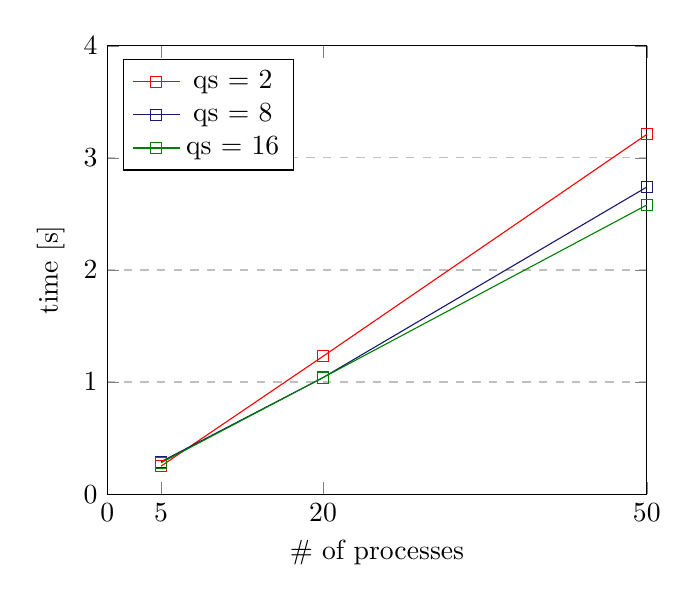
\begin{tikzpicture}
			\begin{axis}[
				ylabel={time [s]},
				xlabel={\# of processes},
				ymin=0, ymax=4,
				xmin=0, xmax=50,
				ytick={0,1,2,3,4},
				xtick={0,5,20,50},
				ymajorgrids=true,
				grid style=dashed,
				legend pos=north west
		]
		 
			\addplot[
				color=Red,
				mark=square,
				]
				coordinates {
					(5,0.25)(20,1.23)(50,3.21)
				};
				\addlegendentry{qs = 2}
	
			\addplot[
				color=MidnightBlue,
				mark=square,
				]
				coordinates {
					(5,0.29)(20,1.04)(50,2.74)
				};
				\addlegendentry{qs = 8}
		
			\addplot[
				color=Green,
				mark=square,
				]
				coordinates {
					(5,0.28)(20,1.04)(50,2.58)
				};
				\addlegendentry{qs = 16}

			\end{axis}
		\end{tikzpicture}
	\end{center}
	\caption{Processing performance}
  \label{fig:processing_performance}
\end{figure}

\subsection{Discussion}
Even though the differences in processing time are quite small, we can deduce from the test results that a \emph{low} quantum size is favorable when running \emph{few} processes and that a \emph{high} quantum size is favorable when running \emph{many} processes. When implementing a dynamic quantum size, although based on a somewhat weak foundation, this suggests changing the quantum size from $ 2 \rightarrow 8 $ when the number of processes running exceeds 5 and changing it from $ 8 \rightarrow 16 $ when the number of processes running exceeds 20, as shown in Table \ref{tab:dynamic_qs}. In order to do this, we could add some code in \tt do\_fork(message *msg) \normalfont in \tt /usr/src/servers/vm/fork.c \normalfont to check how many processes are running each time we create a new fork. If we cross one of the thresholds suggested in Table \ref{tab:dynamic_qs}, change the quantum size that the child inherits from \tt init \normalfont accordingly. A way to obtain the number of processes currently running---and a possible approach to dynamically chaning the quantum size---is suggested in Appendix \ref{app:fork.c}.

\begin{table}[H]
	\begin{center}
		\begin{tabular}{ r | l }
		{\bf qs} & {\bf\# of processes }\\
		2 & 0-5\\
		8 & 5-20\\
		16 & $ 20 \rightarrow $\\
		\end{tabular}
	  
	  \caption{Dynamic Quantum Size thresholds}
	  \label{tab:dynamic_qs}
	\end{center}
\end{table}

\section{Conclusion}
We have seen that tweaking MINIX 3.1.5 system's memory and process mangement can indeed improve performance.

Different memory allocation algorithms suit different scenarios, so the nature of processing that is to be done on a system must be taken into account before choosing which algorithm to implement.

The test results for the quantum size suggest that the quantum size should increase as the number of running processes increase.

For future reference, a system with \emph{lower} processing power than used here should be used to obtain more noticeable differences in processing performance.

\begin{thebibliography}{4}
	\bibitem{minix_book}
		Tanenbaum, A. et. al 2006,
		\emph{Operating Systems: Design and Implementation 3rd ed.},
		Upper Saddle River,
		Pearson
	
	\bibitem{github}
		\url{https://github.com/hanshenrikk/minix-tweak}
\end{thebibliography}

\clearpage
\appendix
\section{/usr/src/servers/vm/alloc.c -- relevant bits}
\label{app:alloc}
\lstinputlisting[language=c]{alloc-relevant-bits.c}

\clearpage
\section{/usr/src/kernel/fork.c -- relevant bits}
\label{app:fork.c}
\lstinputlisting[language=c]{fork-relevant-bits.c}

\clearpage
\section{memory\_program.c}
\label{app:memory_program}
\lstinputlisting[language=c]{../memory_program.c}

\clearpage
\section{memory\_program\_mixed\_array\_sizes.c}
\label{app:memory_program_mixed}
\lstinputlisting[language=c]{../memory_program_mixed_array_sizes.c}

\clearpage
\section{process\_program.c}
\label{app:process_program}
\lstinputlisting[language=c]{../process_program.c}

\end{document}
